\documentclass[14pt,fleqn]{extarticle}
\RequirePackage{prepwell}

\previewoff 

\begin{document} 
\begin{snippet}
    
    \incorrect
    
    Circle $C_1$ is centered at the origin and has radius $R_1 = 1$. Circle $C_2$ is enclosed entirely inside $C_1$ as shown
    
    \begin{center}
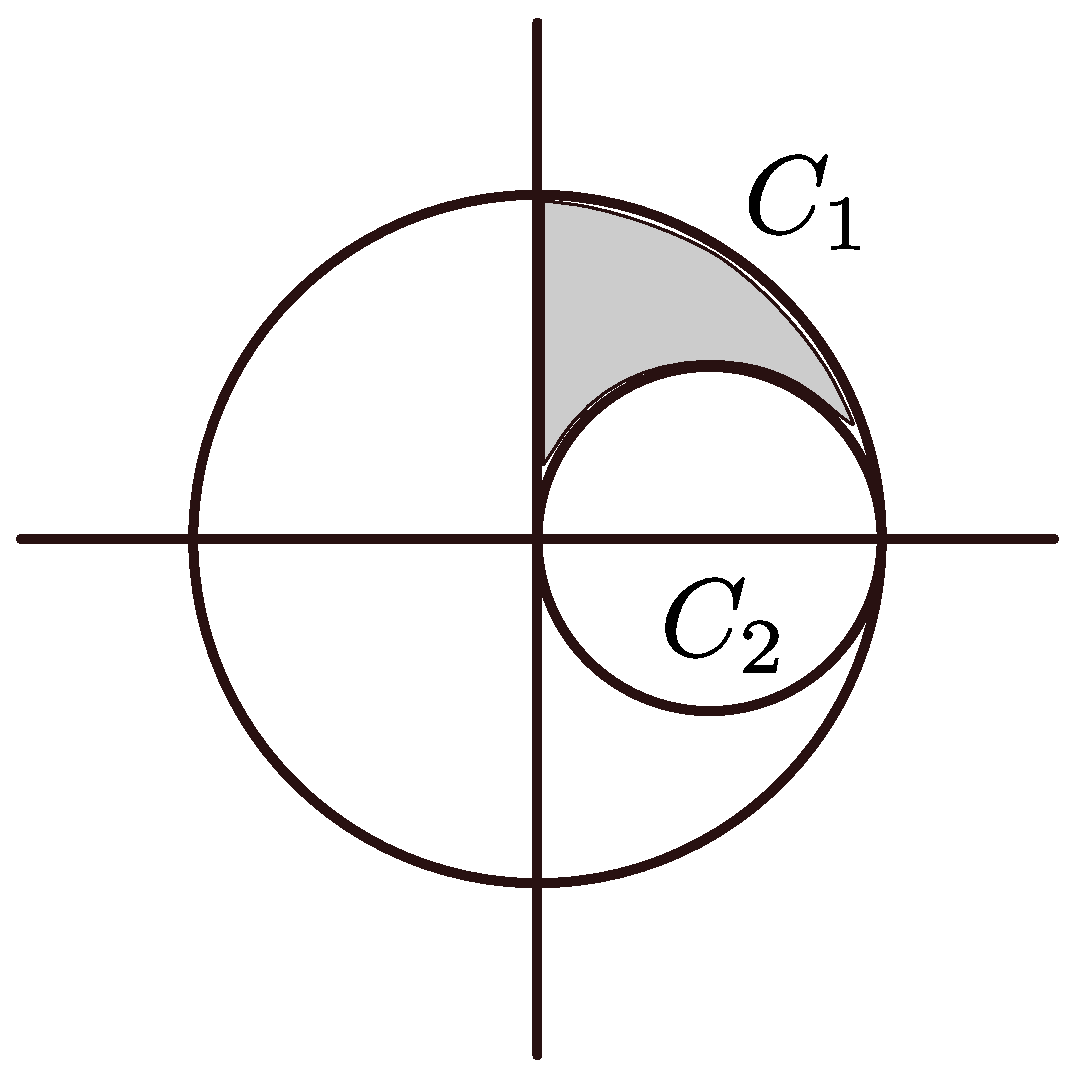
\includegraphics[scale=0.2]{figure.eps}
\end{center}

The area of the shaded region is therefore
\[  A = \int_0^1 \sqrt{1-x^2}\cdot dx - \int_0^1 \sqrt{\frac{1}{4} - x^2}\cdot dx \]
    
    \reason
    
    \begin{center}
  \begin{tabular}{NNNN}
   \toprule
        \text{Circle} & \text{Center} & \text{Radius} & \text{Equation}  \\
   \midrule 
   C_1 & (0,0) & 1 & x^2 + y^2 = 1 \\
    \midrule 
    C_2 & \left(\frac{1}{2},0 \right) & \frac{1}{2} & \left(x-\frac{1}{2} \right)^2 + y^2 = \frac{1}{4} \\
     \bottomrule
  \end{tabular}
\end{center}

And therefore 
\[ A = \underbrace{\int_0^1 \sqrt{1-x^2}\cdot dx}_{\text{Area under }C_1} - \underbrace{\int_0^1 \sqrt{\frac{1}{4} - \left(x-\frac{1}{2} \right)^2}\cdot dx}_{\text{Area under }C_2} \]
    
\end{snippet} 
\end{document} 